\newpage
\section{Incomplete Carbon Pricing Schemes}

% \begin{quote}
% ``You know these pest control companies. They call themselves exterminators, but they can't really do it. The best they can do is get the bugs to go to somebody else's house. They just relocate them, you know what I mean? They're bug realtors is what they are."
% --- Jerry Seinfeld (Seinfeld, Season 6, Episode 19, ``The Doodle")
% \end{quote}

Previously, we have looked at the ability of carbon pricing schemes (either an emissions tax or an emissions trading program) to reduce greenhouse gas emissions within a closed economy. Although this is a standard example of Pigouvian approaches to tackling externalities, the story is more complex when we instead consider an open economy. 

When an individual country/state/city takes up a carbon pricing scheme, we call this a \emph{unilateral} carbon pricing scheme, meaning that this jurisdiction adopts the policy without coordinated carbon pricing schemes across all or most all other jurisdictions. This is the current state of carbon pricing schemes. According to the \cite{wbank}, 21\% of all anthropogenic greenhouse gas emissions faced an emissions price in 2021. Even if Country A has a price on its carbon, it will not be able to put a price on the emissions from Country B, even though Country B's emissions are just as damaging to Country A as its own emissions. That is not to say that unilateral carbon pricing schemes are not worth it, but to acknowledge that there is something missing. This is an example of an \emph{incomplete regulation}: a situation where not all relevant actors in the market face regulation. In the case of greenhouse gas emissions, everyone is a relevant actor, meaning that without a global carbon pricing scheme, any unilateral carbon pricing scheme will always be incomplete. In this section, we begin to explore the implications of the incompleteness of unilateral emissions pricing and analyze possible solutions.

%The fundamental issue that leads to emissions leakage is that unilateral carbon pricing schemes are incomplete forms of regulation. We say that a regulation is incomplete if not all relevant actors in the market face regulation. In a closed economy, a unilateral carbon tax would not induce emissions leakage; all the actors in the market are subject to the carbon tax. This is not the case for the open economies of the real world, prompting the need for additional policies to complement the initial regulation.

\subsection{The Big Picture of Climate Policy \& Competition}

A frequent claim of those opposing aggressive climate policy is that it will make the country less economically competitive relative to other countries.\footnote{Do I dare include something from MTG on this: ``[Supporters of the Green New Deal] want to shut down our economy, they want to end  our energy independence and surrender America, putting us on our knees to China--dependent on China, yes, just to drive a car or a truck. That is not in some distant time in the future. That is pretty soon, especially in less than 10 years\ldots They want to transform America into a Third World country, and that is exactly what these policies will do" \citep{marjorie_greene}.} Here, I will use the term ``competitive" in the sense that foreign firms will gain a greater global market share, usually as a result of lower costs. Understandably, the effect of climate and environmental policy on economic activity (both domestic and foreign) is of considerable interest to not just economists, but policymakers and the general public.

The contemporary literature on the relationship between economic standard of living and environmental decay begins with Simon Kuznets, and his work related not to the environment, but inequality. \cite{kuznets1955economic} laid out a empirical relationship between economic development and inequality. Kuznets findings suggest that income inequality rises as countries move from low-income to middle-income, and income inequality falls as countries move from middle-income to high-income. Diagrammatically, this creates an inverted U-shaped path called the Kuznets Curve with GDP per capita on the horizontal axis and measures of inequality (usually the income ratio between the top quintile and bottom quintile of earners) on the vertical axis. Realizing that economic development and environmental degradation follow a similar relationship, \cite{NBERw3914} were the first to formulate the \emph{Environmental} Kuznets Curve (EKC) in an analysis of NAFTA. While the model was not the primary focus of the original paper, it later led to its own published paper, \cite{grossman1995economic} and is now a standard in environmental economics. 

Figure \ref{EKC} displays the Environmental Kuznets Curve. The EKC hypothesizes that low-income economies will have relatively high environmental quality, as these economies may be more agrarian or pastoral. Countries often move from low-income to middle-income through industrialization, and as countries industrialize, their environmental degradation increases. Eventually though, economic development requires countries to move away from manufacturing and into higher human capital industries. When this happens, sectors dependent on high human capital (e.g., finance, engineering, education) tend to be less harsh on the environment. Past the turning point, economic development will decrease environmental degradation. 

\begin{figure}
\centering
\begin{minipage}{0.48 \textwidth}
\caption{The EKC \label{EKC}}
\begin{tikzpicture}[scale = 0.6]
\draw[thick, <->] (0,10) -- (0,0) -- (10,0);
\draw[thick, EAPblue]  [domain = 1:9] plot (\x, {8.5 - .5*(\x - 5)^2});
\node [below right] at (7,0) {GDP/Capita};
\node[rotate=90, above] at (0,7) {Environmental Degradation};
\draw[dashed] (5,0) -- (5,9.5) node[right]{\footnotesize Turning Point};
\end{tikzpicture}
\end{minipage}
\begin{minipage}{0.48\textwidth}
\centering 
\caption{Application of the  EKC}
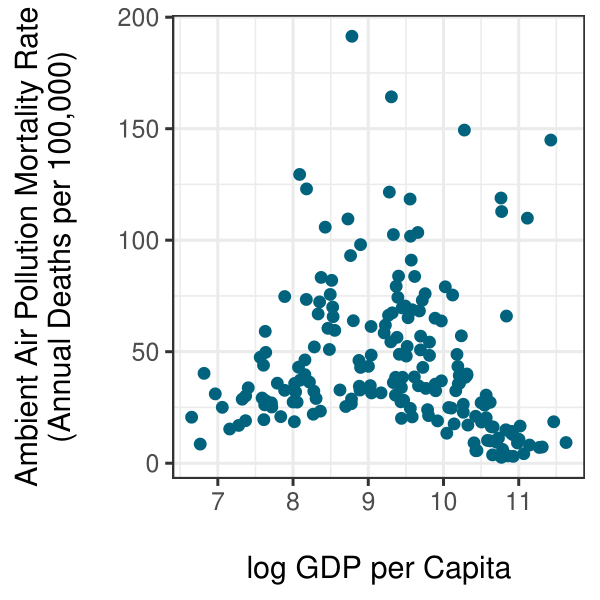
\includegraphics[width=0.9\textwidth]{figures_3/ekc.png}
\end{minipage}
Data from \cite{owidoutdoorairpollution} 
%https://ourworldindata.org/outdoor-air-pollution#outdoor-air-pollution-tends-to-rise-with-industrialization-before-falling
\end{figure}

Despite its quick adoption in the discipline and its continued use, the EKC has largely been discredited \citep{stern2004rise}. \cite{arrow1995economic} importantly note that the usual form of the EKC does not allow for any feedback between the environment and development, implicitly assuming that pollution and other forms of environmental degradation do not hinder economic development. 

The claim from the EKC that economic development itself will lead to improvements in environmental quality make dubious assumptions. The EKC correctly captures the tendency for rich nations to substitute dirty economic activities for relatively cleaner activities. Ultimately though, the world is finite, and some countries must house the high-pollution industries. This leads to what is known as the \emph{pollution haven hypothesis}. Stringent environmental regulation will raise the costs of firms in high-pollution industries, making firms in less-regulated economies relatively cheaper and more competitive. This means that some economies with relaxed environmental regulation might end up specializing in only high-pollution industries, becoming pollution havens. Thus, one consequence of environmental regulation may be that it shifts the burden of damaging economic activities elsewhere, usually to low- and middle-income countries. 

Contemporary empirical evidence on the pollution haven hypothesis leads to a few key conclusions: (1) environmental regulation does not have an economically significant effect overall trade flows, and (2) environmental regulation can have an economically significant effect on the trade flows of specific industries. A common technique for assessing differences in climate policies is considering differences in energy prices \citep[see for example][]{fowlie2022mitigating}. The idea is that carbon prices function in the short-run by raising the price of energy that a firm's technology limits them to use. Using differences in energy prices as a proxy, \cite{sato2015asymmetric} show that an increase in the energy price gap between trading countries only increases bilateral manufacturing trades by 0.2\%. Further these same energy price differences only explain 0.01\% of the variation in trade flows. \cite{aldy2015competitiveness} find a null result in a similar study looking at energy price differences between US states---the effect of energy price differences on total manufacturing imports between states was statistically insignificant, even with their over thirty years of panel data. However, they do find pronounced effects in certain, energy intensive sectors including steel, industrial chemicals, and cement. In their survey of the literature, \cite{dechezlepretre2020impacts} come to the conclusion that there is likely a pollution haven effect, but that it is confined to a select number of industries.

\subsection{Emissions Leakage}

If empirical evidence seems to suggest that climate policy only leads to significant competitive effects in a few industries, where is the problem? Unfortunately, even if the transfer of economic activity is small overall, the transfer of emissions can be quite large.

\emph{Emissions leakage} occurs when the implementation of stringent regulation (almost always meaning a carbon pricing scheme) on GHG emissions in one place leads to increased GHG emissions in another place with looser regulations. Emissions leakage is closely related to the pollution haven hypothesis, but differs in a few ways. First, emissions leakage refers exclusively to GHG emissions, not pollution in general. This distinction is important as most GHG emissions have a negligible effect on the areas downwind from their source of emissions, but ambient air pollutants do not. Thus, the consequences of increased GHGs from emissions leakage is global rather than local. Second, the pollution haven hypothesis is much more concerned with international trade flows and the changing composition of economies, whereas emissions leakage is concerned more with changing the distribution of emissions. That is, the pollution haven hypothesis focuses on the implications of displaced economic activity, and emissions leakage focuses on the implications of displaced emissions.

\begin{figure}
\caption{Competitive Emissions Leakage \label{leakage_ex}}
\centering
\singlespacing
\footnotesize
\begin{tikzpicture}[scale = 0.5]
	\draw[very thick, <->] (0, 11) node[left]{$p$} -- (0, 0) -- (11, 0) node[below, text width = 2cm]{Domestic Quantity};
	\draw[very thick, <->] (15, 11) node[left]{$p$} -- (15,0) -- (26, 0) node[below, text width = 2cm]{Imported Quantity};
	\fill[yellow!80!, opacity = 0.6] (3.5, 3.75) -- (3.5, 1.75) -- (4.5, 2.25) -- (4.5, 4.25) -- cycle;
	\fill[yellow!80!, opacity = 0.6] (4.5, 2.25) -- (5.5, 2.75) -- (5.5, 4.75) -- (4.5, 4.25) -- cycle;
	\fill[orange!80!, opacity = 0.6] (16.75, 4.75) -- (16.75, 2.75) -- (17.75, 3.75) -- (17.75, 5.75) -- cycle;
	%\fill[orange!80!, opacity = 0.6] (16.25, 4.25) -- (16.25, 2.25) -- (16.75, 2.75) -- (16.75, 4.75) -- cycle;
	\fill[red!80!, opacity = 0.6] (21.25, 9.25) -- (21.25, 7.25) -- (22.25, 8.25) -- (22.25, 10.25) -- cycle;
	%\fill[red!80!, opacity = 0.6] (20.75, 8.75) -- (20.75, 6.75) -- (21.25, 7.25) -- (21.25, 9.25) -- cycle;
	\draw[very thick, EAPblue] (0,0) -- (10, 5) node[right]{MC$_d$};
	\draw[very thick, EAPgreen] (0,2) -- (10, 7) node[right]{MC$_d$ $+$ Tax};
	\draw[very thick, gray] (0, 10) -- (10,0) node[pos=.2, above right,text width = 1.5cm]{Domestic Demand}; 
	\draw[very thick, EAPred] (0,5.5) -- (9, 1) -- (10, 0) node[pos=.8, above right, text width = 1.5cm]{Residual Demand};
	%\draw[very thick, EAPred] (0, 6.5) -- (7,3) -- (10, 0);
	\draw[very thick, gray] (15, 10) -- (25, 0) node[pos=.8, above right,text width = 1.5cm]{Domestic Demand}; 
	\draw[very thick, EAPblue] (15, 1) -- (24, 10) node[right, text width = 1.5cm]{MC$_f$};
	\draw[dashed, thick] (5.5, 4.75) -- (5.5, 0) node[below, yshift = -3pt]{$q_d$};
	\draw[dashed, thick] (3.5, 3.75) -- (3.5, 0) node[below]{$q_d'$};
	%\draw[dashed, thick] (4.5, 4.25) -- (4.5, 0) node[below]{$q_d''$};
	\draw[dashed, thick] (0, 3.75) node[left]{$p'$} -- (21.25, 3.75);
	\draw[dashed, thick] (0, 2.75) node[left]{$p$} -- (22.25, 2.75);
	%\draw[dashed, thick] (0,4.25) node[left]{$p''$} -- (20.75, 4.25);
	\draw[dashed, thick] (16.75,4.75) -- (16.75, 0) node[below, yshift = -3pt]{$q_f$};
	\draw[dashed, thick] (17.75, 5.75) -- (17.75, 0) node[below]{$q_f'$};
	%\draw[dashed, thick] (16.25, 4.25) -- (16.25, 0) node[below]{$q_f''$};
	\draw[dashed, thick] (22.25, 10.25) -- (22.25, 0) node[below, yshift = -3pt]{$q$};
	\draw[dashed, thick] (21.25, 9.25) -- (21.25, 0) node[below]{$q'$};
	%\draw[dashed, thick] (20.75, 8.75) -- (20.75, 0) node[below]{$q''$};
	\draw[dotted] (15, 3) -- (23, 11) node[right]{MC$_f$ $+$ Tax};
	\draw[thick, <-] (5, 4) -- (8, 8) node[above, text width = 2cm, align=center]{Domestic Abatement};
	\draw[thick, <-] (17.4, 4.5) -- (18.2, 8) node[above, text width = 2cm, align=center]{Emissions Leakage}; 
 	\draw[thick, <-] (21.7, 8.2) -- (23, 6) node[below right, text width = 1.6cm, align=center]{Net Abatement};
 	\node at (5.5, 12) {Domestic Market};
 	\node at (20.5, 12) {Import Market}; 
\end{tikzpicture}
\end{figure}

Figure \ref{leakage_ex} displays how competitive effects can drive emissions leakage in an example market. In the left panel of figure \ref{leakage_ex} is the domestic market for an emissions creating good. In the right panel of figure \ref{leakage_ex} is the import market for the same good. Domestic producers do not face the full domestic demand curve, as foreign producers will also be willing to supply the domestic market. Instead, domestic producers face the residual demand curve, the difference between the domestic quantity demanded and the import supply at each price. Domestic firms will produce where their marginal cost curve MC$_d$ intersects residual demand. This price then caries into the import market, and foreign firms will produce where the domestic market price intersects their marginal cost curve MC$_f$. Absent any carbon pricing scheme, domestic firms produce $q_d$, foreign firms import $q_f$, and the total market quantity is $q$. 

Now suppose that domestic policymakers implement a carbon pricing scheme. For ease, assume that this takes the form of a per ton emissions tax and that marginal emissions and marginal damages from emissions are both constant. The carbon pricing scheme is unilateral, meaning that it applies to all domestic producers, but not any foreign producers. The constant marginal emissions rate and per unit carbon tax imply that domestic firms pay a constant per unit tax on their output, creating a parallel shift up in from MC$_d$ to MC$_d$ $+$ Tax. Again, firms produce where the marginal cost they face equals residual demand. This causes the domestic price of the good to rise to $p'$ and the domestic production of the good to fall to $q_d'$. The yellow region of left panel in figure \ref{leakage_ex} represents a monetary measure of domestic abatement. If the tax on emissions is set to the social cost of a ton of emissions, then this area is the monetary value of all domestic emissions abatement $\tau E_d$, where $E_d$ is the sum of domestic emissions in the market. Like we should expect, the carbon pricing scheme induces domestic reductions in GHG emissions.

Unfortunately, this is not the case in the import market. Unlike firms in the domestic market, foreign firms do not face this same emissions price. Higher prices in the domestic market without the counteracting increase in costs induce foreign firms to expand their production from $q_f$ to $q_f'$. Analogous to the yellow area, the orange area in the right panel of figure \ref{leakage_ex} represents the social cost of the additional emissions in the import market. This is emissions leakage: an increase foreign emissions as a result of unilateral carbon pricing. Still, unilateral carbon pricing manages to reduce total emissions despite the leakage. Total quantity in the domestic market falls from $q$ to $q'$, with the area of the red region representing the social value of the net abatement. We see that when we take leakage into account, the emissions reductions are much more modest than what they appeared to from domestic production alone. 

There are a certain class of goods that are particularly susceptible to emissions leakage known as \emph{emissions-intensive and trade-exposed} (EITE) goods. A good is emissions intensive if its production creates a lot of emissions per unit (tons of CO$_2$e/\$). We measure the trade exposure of a good with the ratio of the volume traded domestically (value of imports $+$ value of exports) to the total volume of good that passes through the domestic economy (value of domestic production $+$ value of imports). \cite{fowlie2022mitigating} and \cite{fowlie2016measuring} show that it is not enough to be only emissions intensive or only trade exposed to have a high risk of leakage. Both conditions are necessary to have a substantial risk of emissions leakage. EITE goods include cement, steel, and many industrial chemicals.

The bad news of emissions leakage does not end there. There are many ways that emissions leakage can occur. Using the language of \cite{cosbey2020developing}, we have so far discussed the \emph{competitiveness channel}, where emissions increase outside of the regulated jurisdiction as unregulated producers become more competitive. Another important form of leakage occurs through the \emph{energy market channel}. If the US implemented a stringent tax on GHG from cars, we can expect that the domestic demand of gasoline will fall dramatically as US commuters opt for modes of transportation other than gas-fueled vehicles (e.g., electric vehicles, bikes, public transit). The US is large enough though that this will cause prices to fall in global energy markets, and when fuels like petroleum-based fuels become cheaper, more firms will begin using petroleum-based fuels and creating more emissions elsewhere. These general equilibrium effects that move in and around global energy markets are difficult to address without globally coordinated efforts to ditch fossil fuels. These two channels are thought to be the primary drivers of leakage \citep{branger2014climate}

There are also a few ways where we might see negative emissions leakage. That is, situations where ambitious steps towards abatement in one location spillover into abatement somewhere else. The \emph{income channel} provides another opportunity for negative leakage. If a carbon tax makes people poorer in less-regulated jurisdictions, then this could decrease foreign consumption and production of emissions intensive goods and lower emissions. Of course, this is not a favorable way to reduce emissions. The income channel could operate in the opposite direction as well, raising emissions in places where incomes increase as a result of the incomplete regulation. The more likely form of negative leakage occurs through the \emph{technology channel}. Carbon pricing schemes reduce emissions not just by internalizing the externality, but by providing incentives for the creation of new, cleaner technologies. Producers facing emissions pricing certainly have an incentive to adopt cleaner technologies, but producers outside of the regulated region do not have this same carrot and stick. If these new technologies happen to be more cost-effective than existing technologies, then it is possible that producers would adopt these cleaner technologies and reduce emissions this way. The prospect of negative emissions leakage is overly optimistic as a whole, and empirical evidence to date suggests that negative leakage is negligible compared to the other channels of leakage \citep{winchester2013numerical}.

\subsection{Charges, Rebates, and Permits---Oh My!}

An important approach to completing emissions regulations is through border carbon adjustments. Border carbon adjustments (BCAs) are policies that manipulate the price of goods as they move between jurisdictions with different emissions prices, usually between one place with a carbon price and another without a carbon price. That is, these policies adjust the price of goods based on their carbon emissions (or carbon equivalent emissions) at the border. They come in two major varieties: import taxes (charges) and export (output) rebates

\emph{Import taxes} or \emph{import charges} attempt to complete the regulation of domestic markets by subjecting foreign imports to carbon taxes similar to the carbon taxes domestic producers pay. Import charges are the more relevant of the two major varieties of BCAs, and often we use the term BCA when we just mean import charges. This is largely because we import more EITE goods than we export. 

Figure \ref{import_charge} displays how an emissions charge on imports can reduce leakage. Like in figure \ref{leakage_ex}, suppose that domestic firms pay a constant tax for each ton of their GHG emissions. For simplicity, assume that all producers, domestic and foreign, have a constant, identical emissions intensity. With the unilateral emissions tax and without an import charge, there is substantial domestic abatement---represented by the orange and yellow regions in the domestic market---and there is substantial leakage---represented by the red region in the import market. The total emissions reductions are represented by the violet region in the import market. 

Consider now when policymakers impose an import charge analogous to the domestic emissions tax. Now foreign producers face MC$_f$ $+$ Tax, a parallel shift of their previous marginal cost curve. With the marginal cost curve shifting back in the import market, the difference between the domestic quantity demanded and the quantity of imports supplied increases at every price level. As a result, residual demand in the domestic market shifts up. Setting this new residual demand curve RD$''$ equal to the marginal cost MC$_d$ $+$ Tax, increases the domestic quantity from $q_d'$ to $q_d''$. This means that the value of domestic abatement decreases from the sum of areas of the orange and yellow regions in domestic market to just the area of the yellow region. Although there is modest increase in domestic emissions due to the import charge, there is larger reduction in foreign emissions. The import charge moves foreign production from $q_f'$ to $q_f''$. Previous to the imposition of the import charge, the unilateral emissions tax increased the costs of foreign emissions by the area of the red region in the import market. With the imposition of the import charge though, we see that foreign emissions are actually less than they were in the baseline (no domestic emissions tax and no import charge). The social value of this foreign abatement is give by the area of the region in blue. The total quantity of the good in the domestic market decreases from $q_d'$ to $q_d''$. The additional social value of emissions abatement due to the import charge is given by the area of the green region in the import market.

Import charges bring with them a host of technical challenges that for the most part tie back to one central question: how do we assess the emissions of imported goods? 

\begin{figure}
\caption{Leakage with an Import Charge \label{import_charge}}
\centering
\singlespacing
\footnotesize
\begin{tikzpicture}[scale = 0.5]
	\draw[very thick, <->] (0, 11) node[left]{$p$} -- (0, 0) -- (11, 0) node[below, text width = 2cm]{Domestic Quantity};
	\draw[very thick, <->] (15, 11) node[left]{$p$} -- (15,0) -- (26, 0) node[below, text width = 2cm]{Imported Quantity};
	\fill[orange!80!, opacity = 0.6] (3.5, 3.75) -- (3.5, 1.75) -- (4.5, 2.25) -- (4.5, 4.25) -- cycle;
	\fill[yellow!80!, opacity = 0.6] (4.5, 2.25) -- (5.5, 2.75) -- (5.5, 4.75) -- (4.5, 4.25) -- cycle;
	\fill[red!50!, opacity = 0.6] (16.75, 4.75) -- (16.75, 2.75) -- (17.75, 3.75) -- (17.75, 5.75) -- cycle;
	\fill[EAPblue!50!, opacity = 0.6] (16.25, 4.25) -- (16.25, 2.25) -- (16.75, 2.75) -- (16.75, 4.75) -- cycle;
	\fill[violet!80!, opacity = 0.6] (21.25, 9.25) -- (21.25, 7.25) -- (22.25, 8.25) -- (22.25, 10.25) -- cycle;
	\fill[EAPgreen!80!, opacity = 0.6] (20.75, 8.75) -- (20.75, 6.75) -- (21.25, 7.25) -- (21.25, 9.25) -- cycle;
	\draw[very thick, EAPblue] (0,0) -- (10, 5) node[right]{MC$_d$};
	\draw[very thick, EAPgreen] (0,2) -- (10, 7) node[right]{MC$_d$ $+$ Tax};
	\draw[very thick, gray] (0, 10) -- (10,0) node[pos=.2, above right,text width = 1.5cm]{Domestic Demand}; 
	\draw[very thick, gray] (0,5.5) -- (9, 1) -- (10, 0) node[pos=.5, left, xshift = -2pt]{RD};
	\draw[very thick, EAPred] (0, 6.5) -- (7,3) -- (10, 0) node[pos=.8, above right, text width = 1.5cm]{RD''};
	\draw[very thick, gray] (15, 10) -- (25, 0) node[pos=.8, above right,text width = 1.5cm]{Domestic Demand}; 
	\draw[very thick, EAPblue] (15, 1) -- (24, 10) node[right, text width = 1.5cm]{MC$_f$};
	\draw[dashed, thick] (5.5, 4.75) -- (5.5, 0) node[below]{$q_d$};
	\draw[dashed, thick] (3.5, 3.75) -- (3.5, 0) node[below]{$q_d'$};
	\draw[dashed, thick] (4.5, 4.25) -- (4.5, 0) node[below]{$q_d''$};
	\draw[dashed, thick] (0, 3.75) node[left]{$p'$} -- (21.25, 3.75);
	\draw[dashed, thick] (0, 2.75) node[left]{$p$} -- (22.25, 2.75);
	\draw[dashed, thick] (0,4.25) node[left]{$p''$} -- (20.75, 4.25);
	\draw[dashed, thick] (16.75,4.75) -- (16.75, 0) node[below, yshift = -3pt, xshift = 2pt]{$q_f$};
	\draw[dashed, thick] (17.75, 5.75) -- (17.75, 0) node[below]{$q_f'$};
	\draw[dashed, thick] (16.25, 4.25) -- (16.25, 0) node[below]{$q_f''$};
	\draw[dashed, thick] (22.25, 10.25) -- (22.25, 0) node[below]{$q$};
	\draw[dashed, thick] (21.25, 9.25) -- (21.25, 0) node[below]{$q'$};
	\draw[dashed, thick] (20.75, 8.75) -- (20.75, 0) node[below]{$q''$};
	\draw[EAPred, very thick] (15, 3) -- (23, 11) node[right]{MC$_f$ $+$ Tax};
	%\draw[thick, <-] (5, 4) -- (8, 8) node[above, text width = 2cm, align=center]{Domestic Abatement};
	%\draw[thick, <-] (16.7, 4.5) -- (18, 8) node[above, text width = 2cm, align=center]{Emissions Leakage}; 
 	%\draw[thick, <-] (21.6, 8) -- (23, 6) node[below right, text width = 1.6cm, align=center]{Net  Abatement};
    \node at (5.5, 12) {Domestic Market};
 	\node at (20.5, 12) {Import Market}; 
\end{tikzpicture}
\smallskip
Adapted from \cite{fowlie2016measuring}.
\end{figure}

Before we determine how to assess the emissions of imported goods, it is useful to know how we assess the emissions of domestically produced goods. The GHG Protocol, the internationally recognized leader in GHG emissions accounting standards, sets out three emissions scopes. Figure \ref{scopes} summarizes these three different methods to account for an organization’s emissions \citep{ghg_protocol_2011}. Scope 1 looks at just an organization’s direct emissions, like the GHGs that the organization emits on site. Scope 2 includes all these direct emissions from Scope 1, but also includes indirect emissions associated with energy inputs. For instance, a database center might have relatively low Scope 1 emissions, but if all electric power needed for the database center comes from a coal-fueled plant, Scope 2 emissions would be high. Scope 3 takes this a step further to look at the lifecycle emissions associated with an organization. This includes all the emissions captured by Scope 2, and includes emissions embodied in non-energy inputs and downstream emissions from distribution, processing, use, and disposal of its output. Any domestic emissions pricing program first needs to determine what emissions it will use to assess emissions to firms. It is best practice to assess foreign emissions with the same scope as domestic emissions, and likely violates international trade law to assess emissions using a higher scope for foreign producers \citep{cosbey2020developing}.

\begin{figure}
	\caption{Greenhouse Gas Emissions Scopes \citep{ghg_protocol_2011}\label{scopes}}
	\centering
	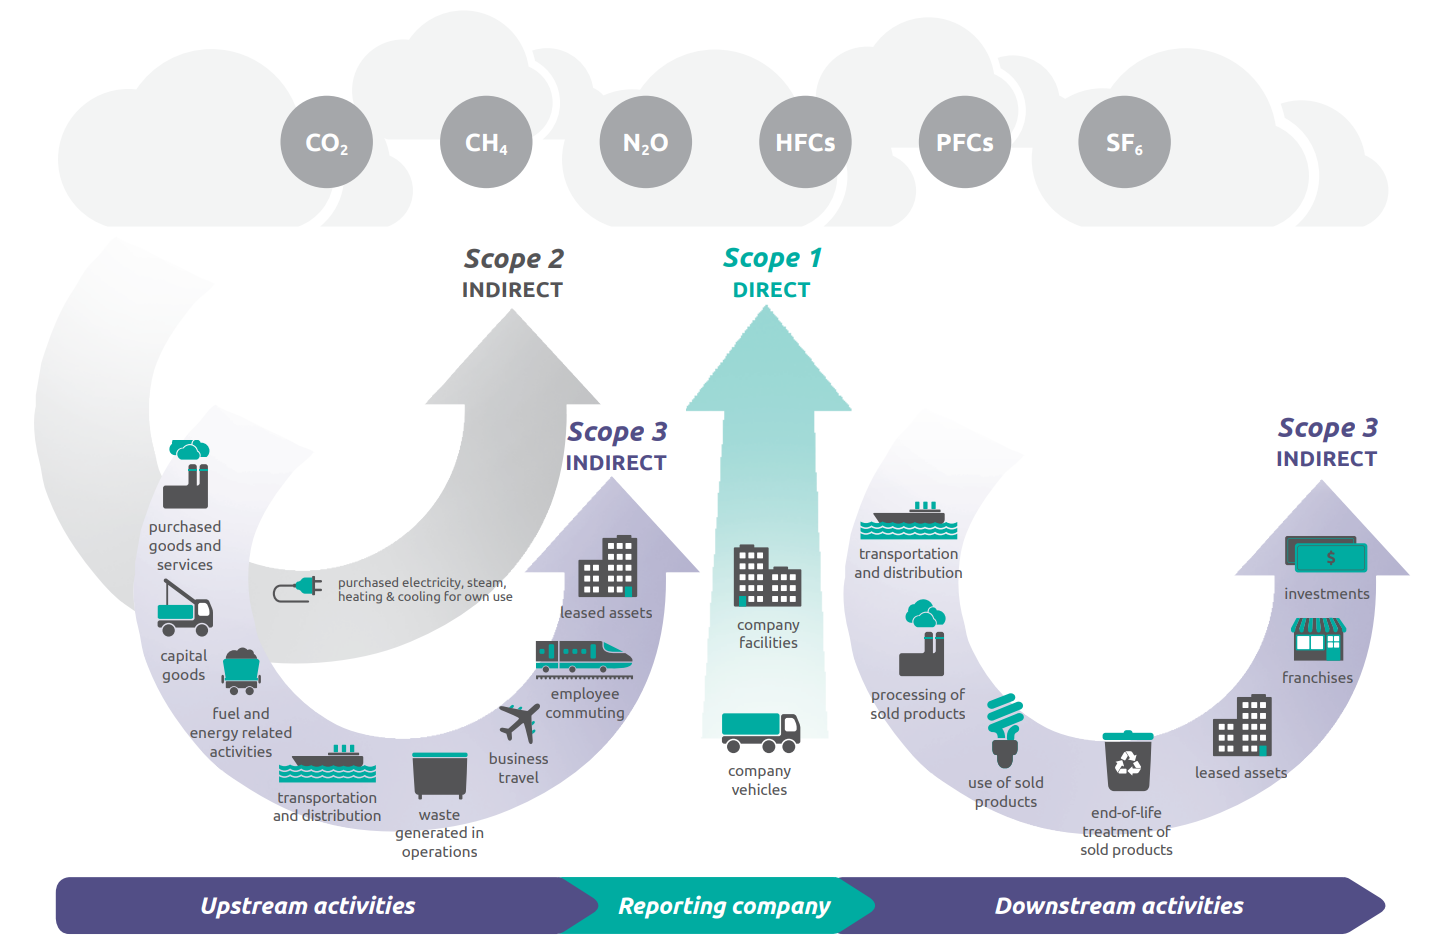
\includegraphics[width=0.8\textwidth]{figures_3/ghg_scope.png}
\end{figure}

In their most complete form, border carbon adjustments cover all goods that cross the border, not just imports. Just like highly-regulated domestic production will likely have a cost disadvantage in the domestic market, highly-regulated exports will likely have a cost disadvantage in foreign markets. To prevent jurisdictions with ambitious climate policy from losing their exports requires some way to adjust the price of exports. This is the purpose of an \emph{export rebate}, often just called an \emph{output rebate}.

An output rebate pays back a flat rate to domestic producers for every unit they export. While carbon taxes on imports try to even the playing field between highly regulated and less regulated producers in domestic markets, output rebates try to even the playing field between highly regulated and less regulated producers on foreign markets. For instance, if US fertilizer manufacturers export much of their product, imposing a domestic carbon tax raises these manufacturers’ costs relative to their competitors overseas. This cost differential may allow foreign fertilizer manufacturers to retake some of the (foreign) market share from US fertilizer manufacturers. This increased foreign production will lead to greater GHG emissions associated with the foreign fertilizer market, a problem that may be exacerbated if foreign manufacturers were already more emissions intensive than US manufacturers.

Output rebates lack the same intuitive appeal that an emissions tax on imports have. After all, why should we tax manufacturers only to pay them back? Why not just tax manufacturers the difference between the original emissions tax and the output rebate? The first reason is a matter of accounting. Output rebates only apply to exports, so reducing the tax on all goods would not differentiate between the goods that should and should not receive a subsidy to avoid leakage. The second reason is a matter of incentives. Output rebates are not refunds on emissions taxes, as the government pays these out for every unit of output rather than for every ton of GHG emissions. In a world where goods had a fixed emissions intensity, this difference would not matter. Thankfully though, there are ways to reduce emissions without reducing output (e.g., switching to cleaner inputs or installing smokestack scrubbers). Thus, an output rebate will maintain the same abatement incentive on exports, while also allowing domestic producers to maintain their ability to compete in foreign markets. The low volume of US manufacturing exports relative to imports means that these are not typically the primary concern in anti-leakage policy.

%\begin{figure}
%\caption{Leakage with an Emissions Tax on Imports}
%\centering
%\singlespacing
%\footnotesize
%\begin{tikzpicture}[scale = 0.5]
%	\draw[very thick, <->] (0, 11) node[left]{$p$} -- (0, 0) -- (11, 0) node[below, text width = 2cm]{Domestic Quantity};
%	\draw[very thick, <->] (15, 11) node[left]{$p$} -- (15,0) -- (26, 0) node[below, text width = 2cm]{Imported Quantity};
%	\fill[orange!80!, opacity = 0.6] (3.5, 3.75) -- (3.5, 1.75) -- (4.5, 2.25) -- (4.5, 4.25) -- cycle;
%	\fill[yellow!80!, opacity = 0.6] (4.5, 2.25) -- (5.5, 2.75) -- (5.5, 4.75) -- (4.5, 4.25) -- cycle;
%	\fill[orange!80!, opacity = 0.6] (16.75, 4.75) -- (16.75, 2.75) -- (17.75, 3.75) -- (17.75, 5.75) -- cycle;
%	\fill[yellow!80!, opacity = 0.6] (16.25, 4.25) -- (16.25, 2.25) -- (16.75, 2.75) -- (16.75, 4.75) -- cycle;
%	\fill[orange!80!, opacity = 0.6] (21.25, 9.25) -- (21.25, 7.25) -- (22.25, 8.25) -- (22.25, 10.25) -- cycle;
%	\fill[yellow!80!, opacity = 0.6] (20.75, 8.75) -- (20.75, 6.75) -- (21.25, 7.25) -- (21.25, 9.25) -- cycle;
%	\draw[very thick, EAPblue] (0,0) -- (10, 5) node[right]{MC$_d$};
%	\draw[very thick, EAPgreen] (0,2) -- (10, 7) node[right]{MC$_d$ $+$ Tax};
%	\draw[very thick, gray] (0, 10) -- (10,0) node[pos=.2, above right,text width = 1.5cm]{Domestic Demand}; 
%	\draw[very thick, EAPred] (0,5.5) -- (9, 1) -- (10, 0) node[pos=.8, above right, text width = 1.5cm]{Residual Demand};
%	\draw[very thick, EAPred] (0, 6.5) -- (7,3) -- (10, 0);
%	\draw[very thick, gray] (15, 10) -- (25, 0) node[pos=.8, above right,text width = 1.5cm]{Domestic Demand}; 
%	\draw[very thick, EAPblue] (15, 1) -- (24, 10) node[right, text width = 1.5cm]{MC$_f$};
%	\draw[dashed, thick] (5.5, 4.75) -- (5.5, 0) node[below]{$q_d$};
%	\draw[dashed, thick] (3.5, 3.75) -- (3.5, 0) node[below]{$q_d'$};
%	\draw[dashed, thick] (4.5, 4.25) -- (4.5, 0) node[below]{$q_d''$};
%	\draw[dashed, thick] (0, 3.75) node[left]{$p'$} -- (21.25, 3.75);
%	\draw[dashed, thick] (0, 2.75) node[left]{$p$} -- (22.25, 2.75);
%	\draw[dashed, thick] (0,4.25) node[left]{$p''$} -- (20.75, 4.25);
%	\draw[dashed, thick] (16.75,4.75) -- (16.75, 0) node[below, yshift = -3pt, xshift = 2pt]{$q_f$};
%	\draw[dashed, thick] (17.75, 5.75) -- (17.75, 0) node[below]{$q_f'$};
%	\draw[dashed, thick] (16.25, 4.25) -- (16.25, 0) node[below]{$q_f''$};
%	\draw[dashed, thick] (22.25, 10.25) -- (22.25, 0) node[below]{$q$};
%	\draw[dashed, thick] (21.25, 9.25) -- (21.25, 0) node[below]{$q'$};
%	\draw[dashed, thick] (20.75, 8.75) -- (20.75, 0) node[below]{$q''$};
%	\draw[EAPred, very thick] (15, 3) -- (23, 11) node[right]{MC$_f$ $+$ Tax};
%	%\draw[thick, <-] (5, 4) -- (8, 8) node[above, text width = 2cm, align=center]{Domestic Abatement};
%	%\draw[thick, <-] (16.7, 4.5) -- (18, 8) node[above, text width = 2cm, align=center]{Emissions Leakage}; 
% 	%\draw[thick, <-] (21.6, 8) -- (23, 6) node[below right, text width = 1.6cm, align=center]{Net Abatement};
% 	\node at (5.5, 12) {Domestic Market};
% 	\node at (20.5, 12) {Foreign Imports}; 
%\end{tikzpicture}
%\end{figure}

\doublespacing

%\subsection*{Border Carbon Adjustments in Practice}